\documentclass{ferseminar}
\setlength{\footskip}{20pt}
\student{Toma Šimunić}
\voditelj{prof.~dr.~sc. Ivana Podnar Žarko, 
	
	mag.ing. Federico-Matteo Benčić}
\mjestodatum{Zagreb}{April}{2018}
\naslov{Implementing cryptocurrency NANO\\ as payment option in e-commerce}
\usepackage{graphicx}
\usepackage{placeins}

\graphicspath{ {images/} }
\begin{document}
\stvoripredstranice
\section{Introduction}
Commerce is an activity of buying and selling. Currencies are arbitrary representations of value which are used in commerce since prehistoric ages. The evolution of currencies can be described in a linear progression:

\begin{enumerate}
	\item Early currencies
	\item Coinage
	\item Paper money
	\item Digital currencies
\end{enumerate}

Blockchain technology and the Proof of Work concept made decentralized digital currencies possible. With the emergence of decentralized digital currencies, hereinafter referred to as cryptocurrencies, some e-commerces started implementing different cryptocurrencies as payments options. Due to their price volatility, cryptocurrencies present a risk to the merchant, but on the other hand provide a few reasons for adopting the new payment option.

One of the motivations for implementing cryptocurrency payment options is to attract new customers by providing a new solution. Cryptocurrency enthusiasts often look for shops that accept their currency and shops gain loyal customers this way. Another, and more important motivation, is that the fees for processing transactions are much lower using some cryptocurrencies than conventional card payment options.

The first and most popular cryptocurrency, Bitcoin, was released in 2009 as an open-source software by Satoshi Nakamoto. Since then, Bitcoin has gained a lot in value and has seen some adoption by e-commerces, as well as regular commerces. The increase in Bitcoin's price had a negative impact on it's adoption as a currency because it resulted in transaction fees rising above those of using most other online payment options. This phenomenon has increased the need for an alternative solution.

Cryptocurrency Nano was first introduced in 2014. It stands out from other cryptocurrencies for having feeless and instant transactions, which is made possible by using the block-lattice structure. This makes it a viable contestant for use in e-commerce.

This paper will analyze and compare conventional payment processing, payment processing using a third-party and Peer-to-Peer payment processing using PayPal, Bitcoin and Nano as examples.


\section{E-commerce payment systems}

Consumer spending via the internet has seen a significant increase in the last decade. By expanding their business online, merchants increase their market reach. Online payment systems can be broadly defined as the means and processes involved in conducting transactions online \cite{Lowry}. Advantages of paying online include:
\begin{itemize}
	\item improved cash flow efficiency - websites are a cost effective way of collecting funds
	\item guaranteed transactions - payment providers offer customers assurance by maintaining high-quality equipment and implementing protection policies to gain trust
	\item reduced cost - online payments reduce cost on both the business and client side of a transaction
	\item increased protection of sensitive information - decreases chance of internal employee fraud
	\item increased protection of merchants - online payment providers assume the risk of fraud
\end{itemize}

The possibility of fraud makes security a priority in online payment systems. Most important security aspects are: identification, confidentiality, privacy, authentication, data integrity, non-repudiation, authorization and customer solvency.

While being an e-commerce has it's advantages, it also has it's price. Merchant's discount is a term used in commerce, both online and offline, to represent the fee that is being payed to the payment processors. The merchant deducts the fee from the price of the product. With most payment processors it averages in range between 1 - 3\%. That is the cost of having secure credit card payments, both online and offline. 

There are three major types of online payment systems:
\begin{enumerate}
	\item conventional payment processing
	\item third-party payment providers
	\item Peer-to-Peer payment
\end{enumerate}

\subsection{Conventional payment processing}
To accept an online payment, a merchant has to obtain an account from a bank and establish an agreement with a payment processor, such as Visa or Mastercard. The components interacting are customer, merchant, merchant's bank and credit or debit card issuer.

A \textbf{merchant's account} is a bank account capable of receiving funds from his online customers. 

A \textbf{credit or debit card issuer} is the company which issued the card to the customer. When the transaction is in the authorization phase, the payment processor is using the card company's network to determine whether the transaction is valid.

\textbf{Shopping cart software} is used to maintain a link between a customer and his set of selected items by allowing him to store items in the cart. It serves as a link between the merchant, customer and the payment processor.

A \textbf{payment gateway}, connects the shopping cart with the merchant's bank and the customer's bank and as a communciation channel between the customer, merchant and the payment processor. The payment processor communicates with the financial networks to determine whether to authorize the transaction. 

The customers selects what he wishes to buy. The items he selected are saved in the shopping cart. When the customers wishes to conclude his order, he gives his card information to the shopping cart software which forwards that information to the payment gateway. The payment gateway verifies the card information with the payment processor. If everything is confirmed, an approval is sent to the payment gateway which communicates the confirmation with the shopping cart. Then, a payment settlement is initiated to transfer funds from the customer's to the merchant's account. 

The whole process consists of two parts:
\begin{enumerate}
	\item authorization
	\item settlement
\end{enumerate}

The \textbf{authorization} part start with the customer confirming his order and finishes with the payment processor notifying the customer that his order has been accepted.

The \textbf{settlement} part starts periodically to send the amount that is owned by the issuing account to the acquiring account. 

The whole Conventional payment process model is represented in Figure 1.

\begin{figure}[p]
	\caption{Conventional payment processing diagram}
	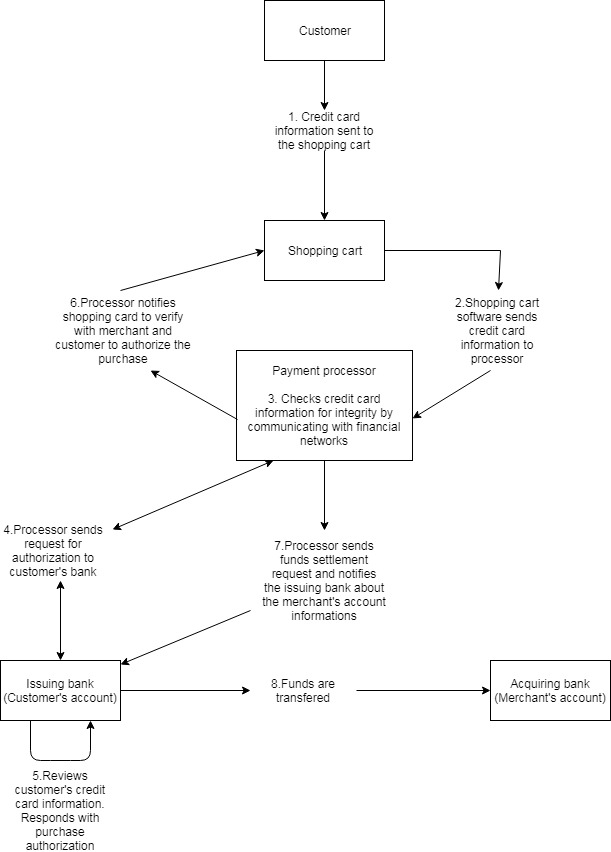
\includegraphics[scale=0.7]{diagram1}
	\centering
\end{figure}

\FloatBarrier

\subsection{Third-party payment providers}

The third-party online payment process is similar to the conventional payment system. In this system, the third-party processes all the transaction funds so there is no need for a merchant account. The system is shown in Figure 2. 

The \textbf{shopping cart} is still responsible for maintaining a connection between the customer and the selected items. When finished shopping, the customer is forwaded to a webpage maintained by the third-party payment provider to collect credit card information.

The \textbf{payment gateway} authorizes the transaction and holds the funds in trust for the merchant. Transfer to the merchant's local bank account occurs on a regular basis, predetermined in the subscription contract.

Modern services that could be categorized as third-party payment providers are \textbf{Google pay} \cite{Google}, \textbf{Apple pay}, \textbf{PayPal} and \textbf{Shopify}. PayPal, while being a third-party payment provider, uses a different business architecture which will be explained in the next section.

\begin{figure}[ht]
	\caption{Third-party payment processing diagram}
	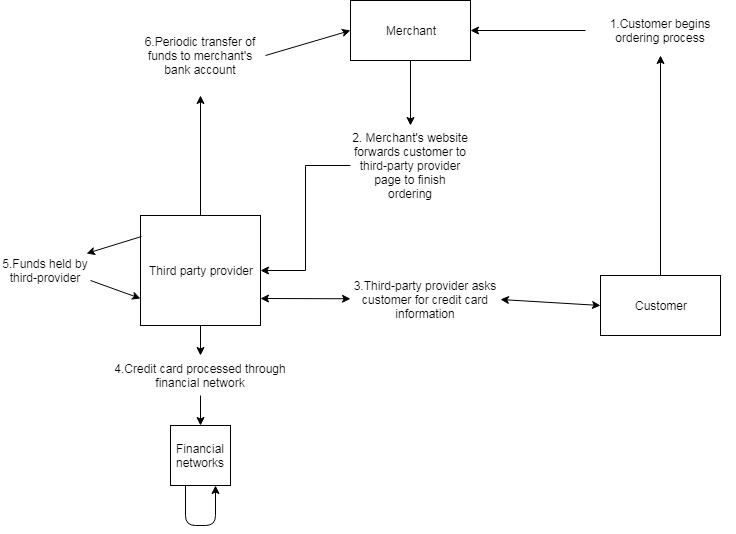
\includegraphics[scale=0.26]{diagram2}
	\centering
\end{figure}
\FloatBarrier

\subsection{Peer-to-Peer payment}

Peer-to-Peer payment is a form of online payment that provides an inexpensive way to accept online payment services. PayPal is recognized as the most prominent among the P2P payment services. PayPal was established in 1998 and is owned by eBay since 2002. For a P2P service to work, both the merchant and the customer need to have an account with the same P2P provider because the payment process is handled internally through the P2P provider. Figure 3 shows a typical P2P transaction.

There are a few differences between PayPal's P2P solution and cryptocurrencies. First, PayPal uses a fee equaling around 3\% plus a small fixed amount per transaction while cryptocurrency fees are not percentage fees and are not dependent on the amount being sent or they have no fees, as shown in the case of Nano. The second difference is that PayPal is directly connected to their users bank accounts or credit / debit card acounts to charge users while trading with cryptocurrencies is direct from the customer's to the merchant's cryptocurrency wallet. Both systems require high-level security management. The difference is that in the Nano network the protocol provides security while in the PayPal network the security and risk management is provided by the web service. That is the reason why PayPal fees are generally higher than cryptocurrency fees.

\begin{figure}[ht]
	\caption{Peer-to-Peer payment processing diagram}
	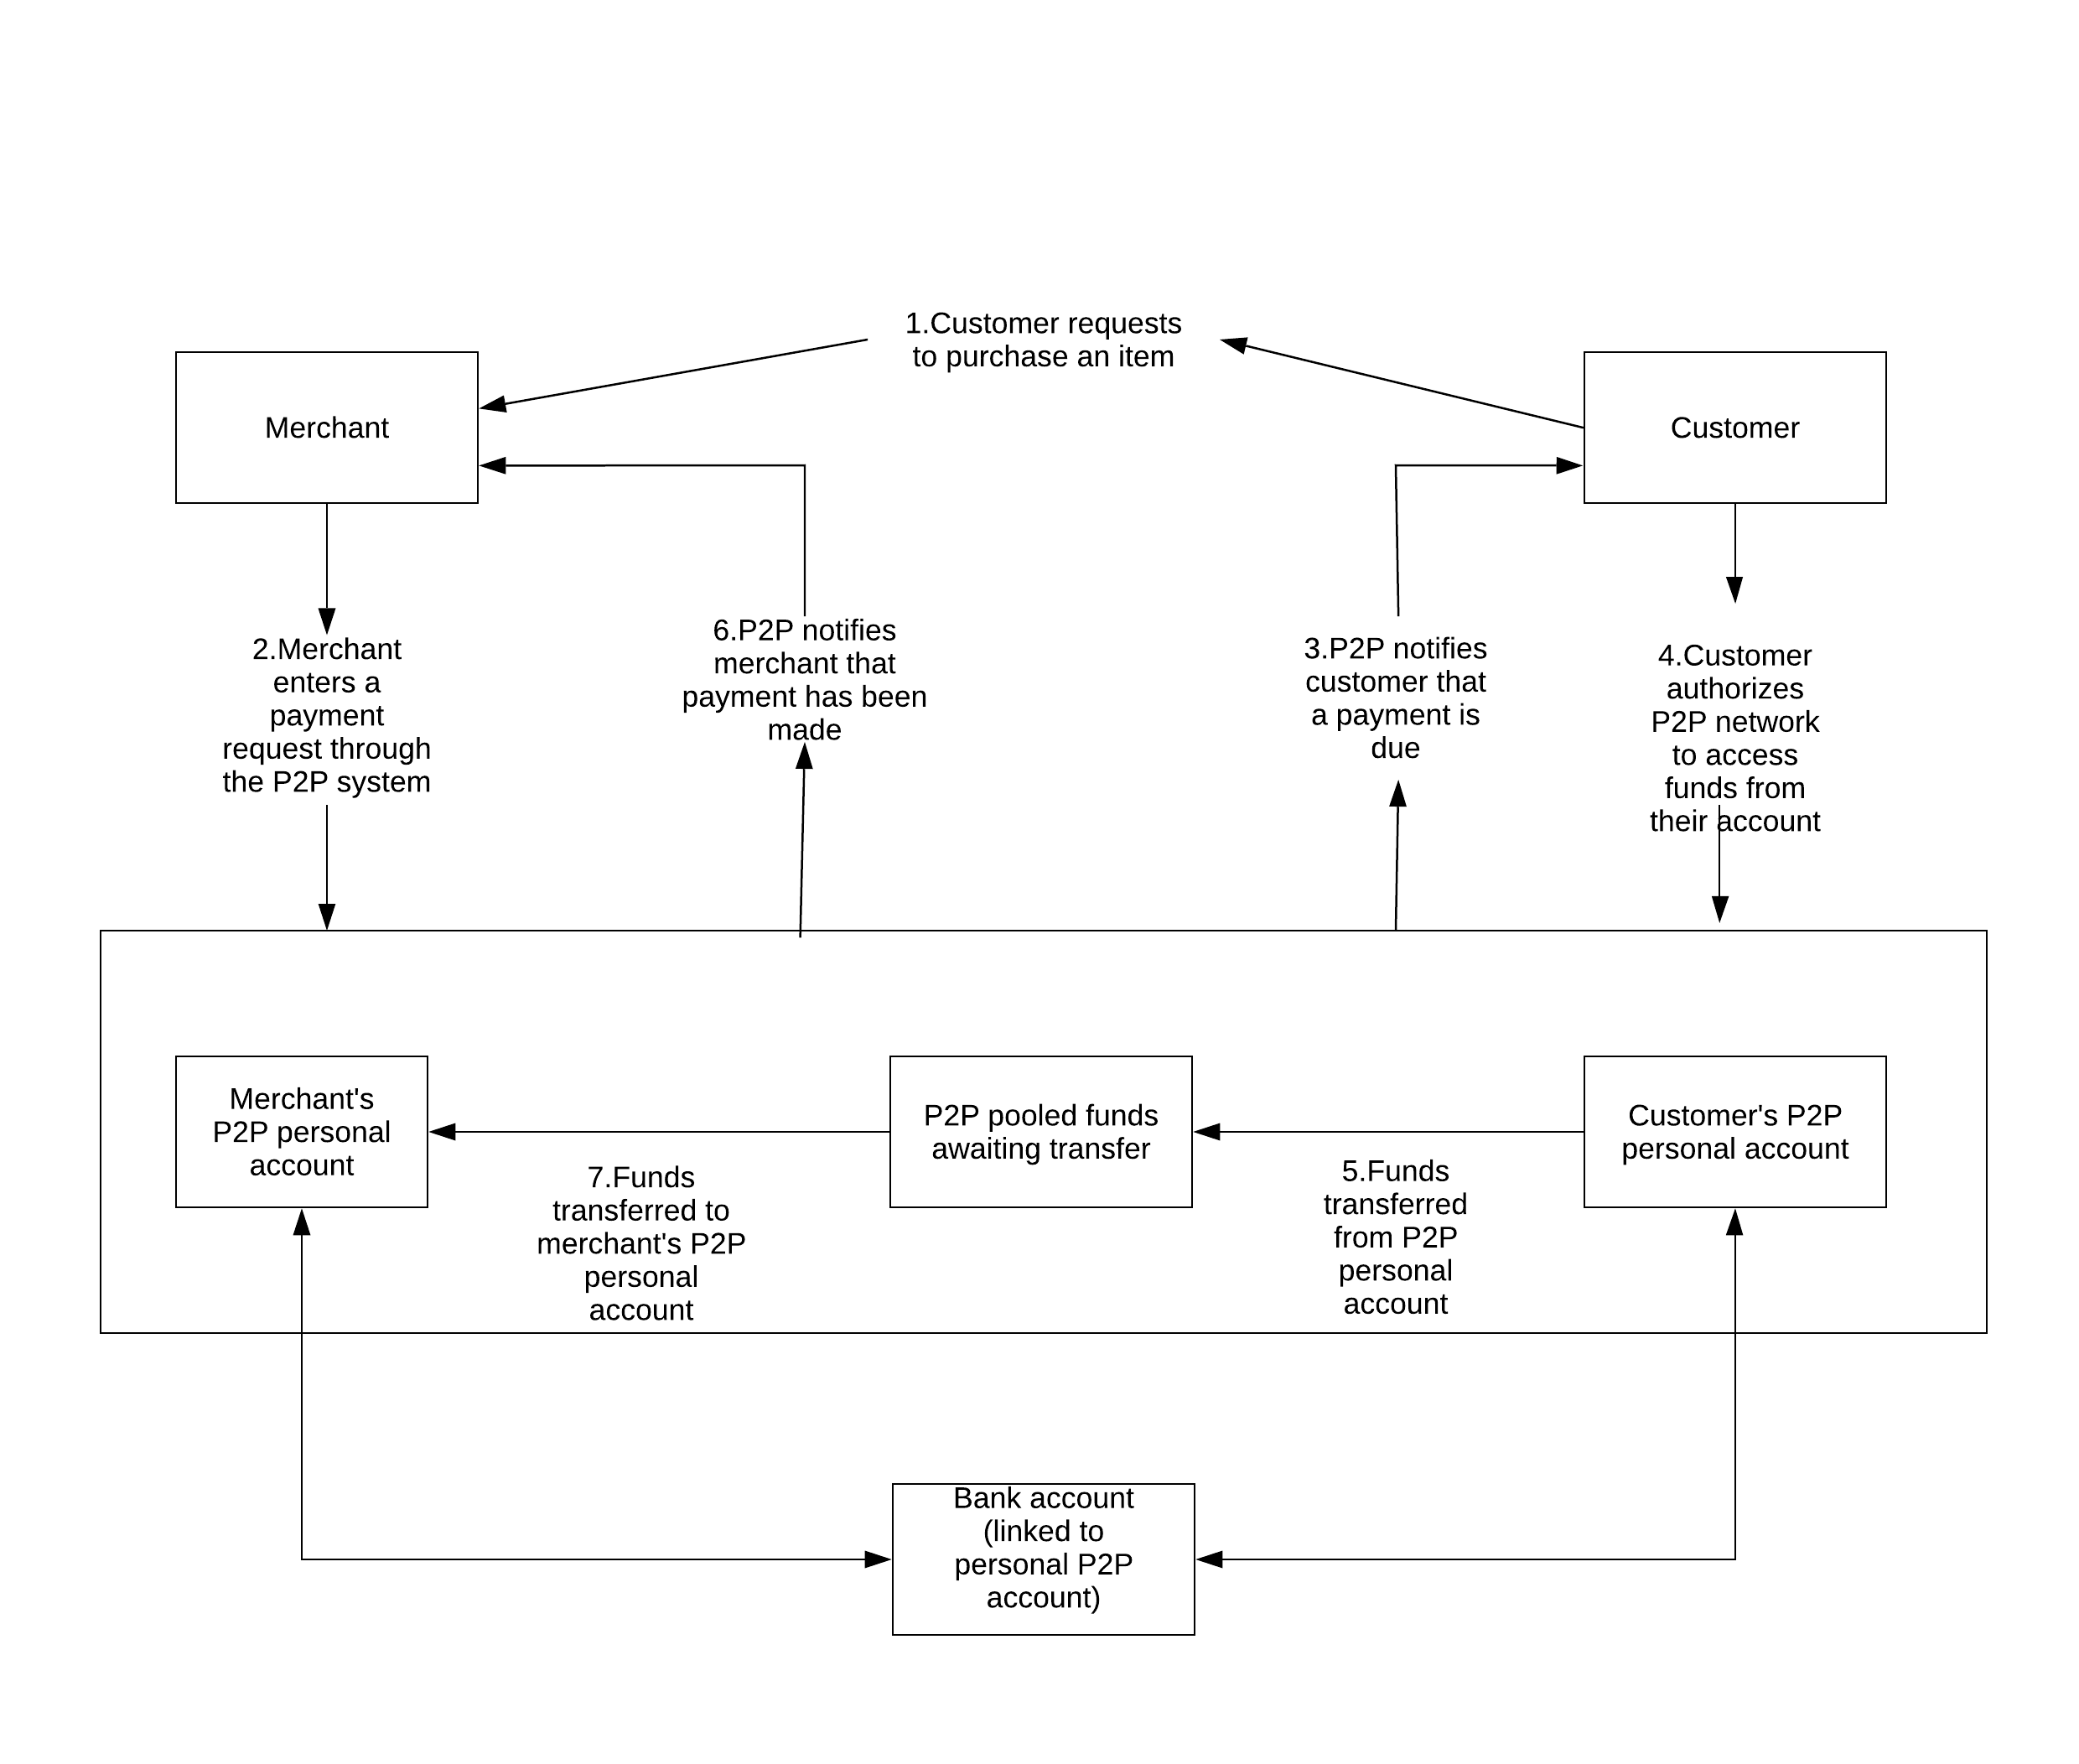
\includegraphics[scale=0.19]{diagram3}
	\centering
\end{figure}
\FloatBarrier

\section{Bitcoin in e-commerce}

Bitcoin is a cryptocurrency developed by Satoshi Nakamoto and published as an open-source software in 2009. It uses a blockchain data structure for storing transaction information and a Proof of Work consensus protocol to secure the validity of the transactions, making them tamper-proof. It allows online payments to be sent directly, peer-to-peer, without going through a financial institution and the consensus mechanism is based on cryptographic proof instead of third trusted party \cite{Bitcoin}.

When Bitcoin was first introduced, it was proposed as a solution to online payments without requiring an intermediary between the customer and the merchant, cutting the costs of transactions in the process. This was favourable to both customers and merchants, which made it popular in e-commerce. However, for the payments to be processed a checkout application must be in place to monitor the payment for the specific products. This requires either programming skills to develop a payment processor or a third-party payment processor. The payment process is similar to the one described in Figure 3 without using bank accounts. Instead, both the merchant and the customer are the primary owners of their accounts and therefore settle transactions without bank accounts.

Most recently, Bitcoin has seen a negative adoption trend, it was discarded by the world's largest gaming platform \textit{Steam} \cite{Steam}. Valve, the owners of \textit{Steam}, stated that the reasons were high volatility and high transaction fees. During December, 2017. Bitcoin's fees went up to a price of around 52 USD per transaction, making it a luxury to pay in Bitcoin. Transaction fees have decreased from then on, today being 1.3 USD. This still represents a problem for average Bitcoin users.


\subsection{Bitcoin performance}
Bitcoin's network produces one block every 10 minutes, each transaction has a size of 7761 bytes and each block containing 1 MB. That makes the Bitcoin network average in around 7 transactions per second (TPS). Transactions that have offered the highest processing fee for transactions have a higher chance to be processed first.


\subsection{Third-party payment processors}
Third-party payment processors are services specialized in providing tools to integrate Bitcoin payment option into your website. The most prominent among them are Coinbase, BitPay and BIPS. 

\subsubsection{Coinbase}
Coinbase is a Bitcoin payment processor that offers 0\% fees for the first million USD in transactions and 1\% fee after. It is only available for US bank accounts and offers a simple website integration. Coinbase also serves as a gateway for buying Bitcoin with USD.
\subsubsection{BitPay}
BitPay is an international payment processor for businesses and charities. BitPay works with Amazon, allowing merchants to sell and ship items through Amazon using cryptocurrencies. It requires a 1\% fee or a monthly fee of 3000 USD.
\subsubsection{BIPS}
Short for the Bitcoin Internet Payment System, it allows merchants to buy and sell Bitcoin for 0\% fees. It also offers an easy-to-use mobile checkout app and a point-of-sale for commerces without internet shops.
\subsection{Pros and Cons of using Bitcoin in e-commerce}
\subsubsection{Pros}
There are \textbf{no chargebacks} with Bitcoin payment. Once a transaction is confirmed the funds are transfered and the order shipped.

\textbf{You determine the transaction fees.} Transaction fees are flexible and depend on the busyness of the transaction pool. If your transaction doesn't have the need to be processed quickly, you can pay a much lower fee.

\textbf{Pseudoanonimity.} Bitcoin addresses aren't tied to your identity. However, by thoroughly investigating transactions tied to a particular address, one can determine who is the owner.

\subsubsection{Cons}
\textbf{Price volatility.} Bitcoin, like most cryptocurrencies, is a speculative asset. It can double or halve it's worth in a single day, making either customer or merchant unhappy with the transaction.

\textbf{Security.} Bitcoin is a novelty in the technological worth so there are still ways that can ease the use of it as a currency to the average user. Banks hold your money for a price but offer security. By safekeeping your own money you take the risk of doing so. 

\textbf{Speed.} In the Bitcoin network, one block is mined every 10 minutes, averaging in 7 transactions-per-second. This makes customers wait for 10 minutes, if they prioritize this transaction with high fees, to have their orders confirmed. However, for the transaction to be finalized, at least 6 blocks sequential to the block that contains the specific transaction have to be mined which results in a final confirmation time of 1 hour.

\textbf{Transaction fees.} Transaction fees are volatile and are entirely dependent on mining pools that can raise the fee at any moment. In the cryptocurrency-sphere there is a rule of thumb for establishing if the fees of a currency are too high. If you wouldn't pay for coffee with the currency, the fees are too high. Bitcoin transaction fees over time are presented in Figure 4.

\textbf{Power inefficiency.} The Bitcoin network consumes an estimated 66.98 TWh per year using an average 903 KWh for a transaction \cite{struja}. This is the equivalent of the yearly energy expenditure of the Czech Republic.

\begin{figure}[ht]
	\caption{Bitcoin transaction fees chart \cite{fees}, [\$/date]}
	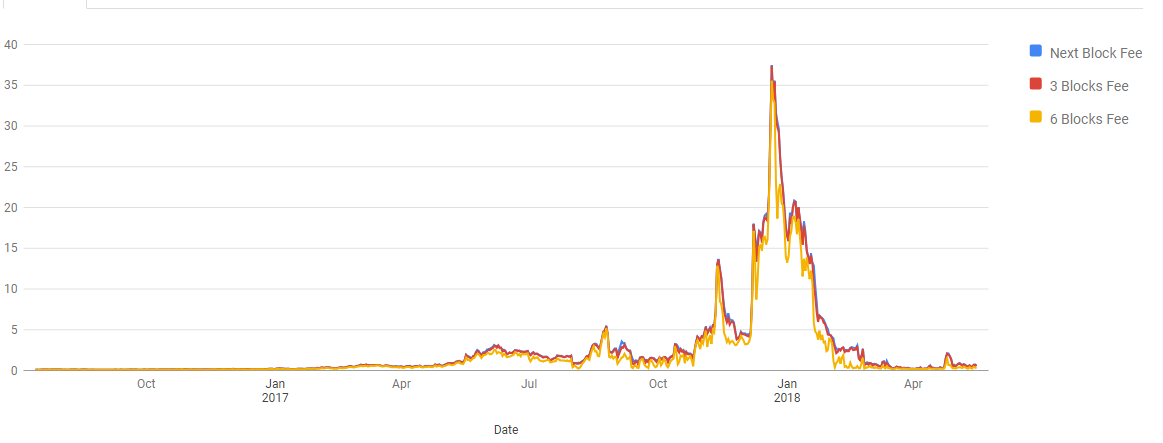
\includegraphics[scale=0.5]{btcfee}
	\centering
\end{figure}
\FloatBarrier

\section{Nano cryptocurrency}

NANO is a low-latency cryptocurrency introduced in December, 2014 as Raiblocks by Colin LeMahieu. It is one of the first Directed Acyclic Graph (DAG) cryptocurrencies built on an innovative block-lattice data structure which offers unlimited scalability and no transaction fees. Nano is a simple protocol by design and only has the purpose of being a high-performance cryptocurrency \cite{Nano}. Nano and Bitcoin differ in many aspects which will be presented in this chapter.

\subsection{Nano components}
The overall Nano architecture consists of four individual components:
\begin{itemize}
	\item Account
	\item Block/Transaction
	\item Ledger
	\item Node
\end{itemize}

An \textbf{account} is the public-key of a digital signature key-pair. The account's public-key also serves as the account's address and is publicly available while the private-key is kept secret. By signing a transaction it is ensured that the contents were approved by the private-key holder and are therefore added to the account's transaction chain. 

In the Nano network each \textbf{block} contains only one \textbf{transaction}. A transaction is an action while the block is the digital encoding of the transaction. These two terms are often used interchangeably since they describe similar terms \cite{Nano}.

The \textbf{ledger} is the global set of accounts where each account has its own transaction chain. This converts a seemingly shared distributed data structure into a non-shared distributed data structure. Each account's transaction chain is stored on Nano network nodes.

A \textbf{node} is a piece of software running on a computer that conforms to the Nano protocol and participates in the Nano network. The node may either store the entire ledger or a pruned history containing only the last few blocks of each account's blockchain. Nodes communicate with each other to update their ledger and to vote on dilemmas that occur in the network.

\subsection{System overview}

Nano uses a block-lattice structure. In the block-lattice structure every account has its own blockchain which is equivalent to the account's transaction history. The account-owned blockchain can only be updated by the private key owner. The nodes in the network are designated to keep the account's balance in check. Some nodes are uninterested in keeping the whole transaction history of an account so they store only the last transactions of every account chain. The last block in an account chain doesn't contain the last transaction information but contains the account balance.

A block is created on the sender's chain to send a certain amount of Nano and a different block is created on the receiver's chain to settle the account's new balance.

Each transaction in the Nano protocol is small enough to fit into a UDP packet. This feature gives the Nano network low-latency. Currently, there are four transaction types: 
\begin{itemize}
	\item open
	\item send
	\item receive
	\item change
\end{itemize}

An upgrade called the \textbf{universal transaction} has been introduced to replace the current four transaction types. It will make each account's blockchain smaller and will allow easier ledger prunning. Prunning is a process of minimizing the ledger size by deleting redundant information. The launch of \textbf{universal transactions} will also increase the overall network performance, lowering the amount of information communicated between nodes.


\subsubsection{Delegated Proof of Stake}

The network reaches consensus via a delegated Proof of Stake (DPoS) voting mechanism. To understand the DPoS voting mechanism, Proof of Stake (PoS) has to be explained. PoS was first presented by PeerCoin \cite{Peercoin} as an alternative to the electricity-inefficient Proof of Work consensus mechanism used by Bitcoin. The next block in the PoS network isn't mined by expensive equipment but is mined by a network participant that is chosen by combining two parameters, coin amount owned by the participant and randomizing.

Delegated Proof of Stake (DPoS) is a PoS variant which includes delegating your account's Nano amount, which represents the users voting power, to a node which will vote on the users behalf. This is useful because the Nano network doesn't have block mining in the conventional sense which will be explained further. 

Nano accounts choose delegates using the change block. Delegate nodes are called representatives in the Nano network. By choosing a representative they delegate their voting power to that particular representative's node. Nano users should pick representatives they trust to avoid someone using their votes to attack the Nano network. A vote is initiated when an account attempts to make a double-spend attack. A double-spend attack happens when an account attempts to spend the same funds more than once. When such an attack happens, the nodes vote on which transaction they will confirm. The remaining transactions are discarded.

Representatives in the Nano network aren't awarded with new Nanos for securing the network. Their incentive for securing the network is that they can use the Nano currency as a payment option for their e-commerce or any other web activity. This provides merchants with an option to enable online transactions for the cost of running a node which is much lower than paying an online payment processor fees ranging from 1-3\% per transaction. The cost of running a node ranges form 10-20\$, depending on the quality of the node that is needed for the specific web activity, and can be accomplished by renting a cloud server and deploying the node software \cite{github}.

\subsubsection{Proof of Work}

For a transaction to be broadcasted to the network, Proof of Work has to be performed. Proof of Work (PoW) is different for the Nano and Bitcoin networks. Bitcoin uses PoW to reach ledger consensus while Nano uses PoW as a spamm prevention tool, similar to HashCash. PoW is performed by hashing the previous block in the account chain. In the Nano network it is performed by the device that is performing the transaction or by a device designated to perform the PoW. The next transaction in an account chain can be pre-mined, since the previous block is already known, which makes transactions appear instantaneous to the end user. This can not be done in the Bitcoin network because a block in the Bitcoin network is a collection of transactions mined by many different actors and the block in the Nano network contains one transaction which can only be broadcasted and mined by the private-key holder.

Nano uses the Blake2b hashing algorithm to perform the work. In the Nano network, the PoW difficulty is set low and is simply used as an anti-spamm tool. The benefit of using a low-difficulty PoW is that transactions seem instantaneous.


\subsection{Nano performance}
Nano offers instantaneous transactions and does that without requesting fees. The Nano test-network scaled to 10000 transactions-per-second while the main-network has been tested on 300 transactions-per-second \cite{Stress}. In theory the scalability is unlimited and in praxis it is limited by the hardware used by the representatives' nodes.

A node requires a voting power equal to 1/1000 of the total voting power to participate in the voting process. This makes the network more secure by not allowing small actors to delay the network with low-performing hardware.

In the Nano network, a transaction is finalized once the nodes, which hold the current state of the ledger, that have 51\% of voting power have the transaction stored in their ledger which happens in a few seconds.

\begin{figure}[ht]
	\caption{visualization of the block-lattice. 
		Every transfer of funds requires a
		send block (S) and a receive block (R), each signed by their account-chain’s
		owner (A,B,C) \cite{Nano}, Nano whitepaper, page 3}
	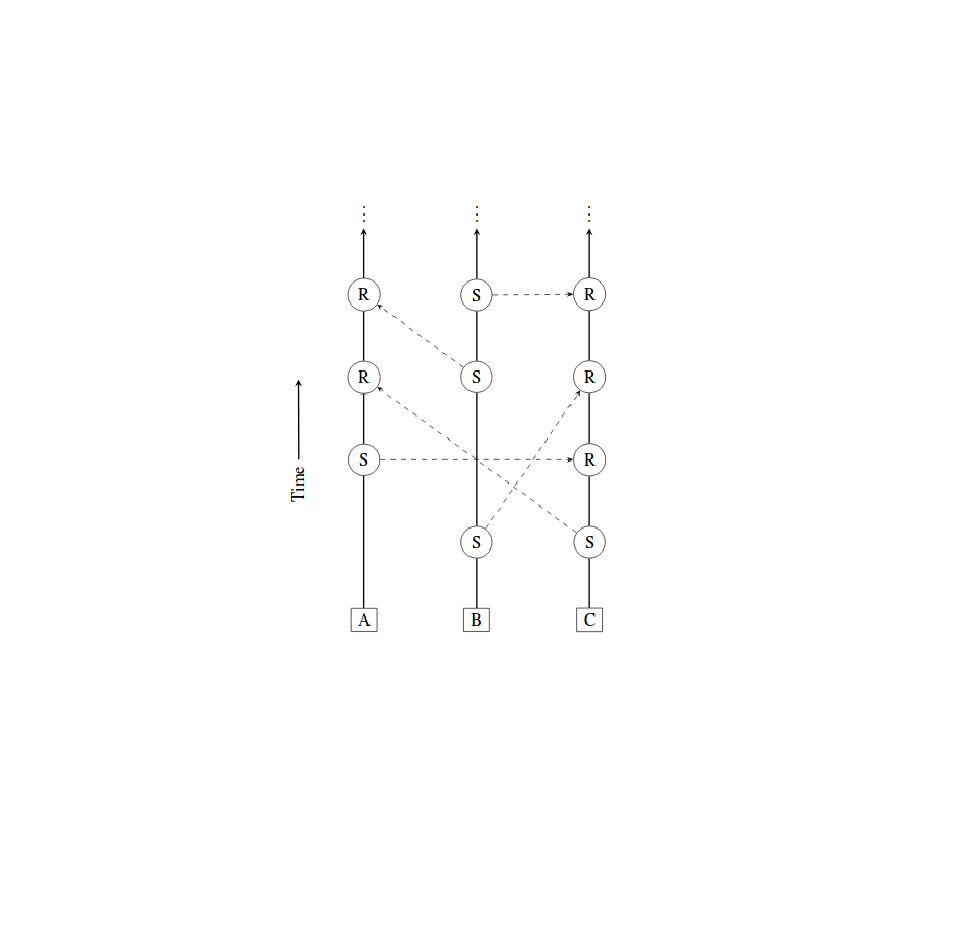
\includegraphics[scale=0.55]{lattice}
	\centering
\end{figure}
\FloatBarrier

\section{NANO in e-commerce}
An analysis of e-commerce trends \cite{Lowry} has shown that there are three areas that can potentially increase the use of online payments:
\begin{itemize}
	\item micropayments
	\item mobile payments
	\item distributed payment systems
\end{itemize}

\textbf{Micropayments} are small electronic payments. The difficulty in implementing micropayments lies in charging transaction fees which can possibly be greater than the payment itself.

\textbf{Mobile payments} are payments made from a mobile phone. Prior to the emergence of smartphones, researchers were investigating the potential use of mobile devices in short range wireless networks for commerce. With current technology, mobile devices have the ability to reach and interact with any website available on the World Wide Web. In addition, many cryptocurrency wallets offer smartphone applications which provides a better solution than the short range wireless networks that were being researched in 2006.  

Leaving a centralized client-server payment system and making a \textbf{Peer-to-Peer distributed electronic system} (P2P) can grant many benefits. The payment processors require fees which can be drastically decreased or removed in a P2P system.

\textbf{Nano} is capable of fulfilling all of those requests. \textbf{Micropayments} are made possible by the non-existence of transaction fees, the low latency of the network and high scalability. \textbf{Mobile payments} will be possible with the final release of the Android and iOS wallets and the development of third-party checkout applications such as Brainblocks \cite{Brainblocks}. The transactions don't need to be mediated by third-parties which in synergy with non-existent fees make it a perfect match for e-commerce use.

By using Nano, a merchant gains a feeless and instant payment option for his online store. This is a feature that currently isn't provided by any other cryptocurrency or payment processor for conventional online payment. The cost of implementing Nano as a payment option is equal to the cost of running a node in the Nano network which is the cost of renting a cloud server. This makes Nano the best payment solution currently available for e-commerces.

To use Nano in an e-commerce, a checkout service must exist to serve as an intermediary for the merchant and the customer to settle the order. Many checkout applications were developed in early 2018 by independent programmer teams. One of them is Brainblocks \cite{Brainblocks}, a feeless payment processing service that can provide checkout services to e-commerces.

Nano faces the same problem as Bitcoin in terms of price volatility. This problem can be solved by implementing a gateway to convert Nano to a conventional currency immediately after settling the transaction. Implementing this solution wouldn't work for Bitcoin due to it having large fees and therefore it would be costly for the e-commerce. 
\subsection{Nano availability}

A currency has to be available to be used. The availability of cryptocurrencies is solved by exhanges. Cryptocurrency exchanges serve as intermediaries between conventional currencies and cryptocurrencies. The requirements of exchanges are:
\begin{itemize}
	\item low fees
	\item legality in their area of operation
	\item security
	\item liquidity
\end{itemize}

In terms of use as a currency, Nano is still in it's early stage and the technology is different than any other distributed ledger technology that cryptocurrencies use. These two things make implementing Nano an issue for most exchanges. Nevertheless, some exchanges have decided to take that step and pave the way for other exchanges. Still, the exchanges that have implemented Nano do not have pairings with conventional currencies and therefore the customer has to buy another cryptocurrency, which has a conventional currency pairing, and then transfer it to an exchange that has Nano implemented. Among the cryptocurrency exchanges that have implemented Nano, the most prominent ones are \textbf{Nanex}, \textbf{Binance} and \textbf{CoinFalcon}.

\subsubsection{Nanex}
Nanex is a non-official Nano cryptocurrency exchange that was developed in early 2018 by an independent programmer. It uses Nano as the primary trading pair making it the first Nano exchange. It has the best uptime percentage which is suggesting it has has a quality implementation of the new cryptocurrency. It has low trading volume but, due to highest uptime percentage, provides the most secure service.

\subsubsection{Binance}
Binance is one of the biggest cryptocurrency exchanges in the world. It has enabled Nano trading in early 2018. Since then, it had shutdown Nano deposits and withdrawals quite a few times due to node fixes and optimizations. It has a higher trading volume than Nanex which makes it a better option for large purchases.

\subsubsection{CoinFalcon}
The first trading NANO/EUR (Nano to Euro) trading pair has been opened on CoinFalcon exchange in May, 2018. Euros can be deposited and withdrawn from CoinFalcon via the SEPA payment protocol. This is an exchange with low volume and therefore still isn't capable of providing optimal services to e-commerces. It charges 1€ for deposits and doesn't charge Nano withdrawals. 
 
\subsection{Payment gateways}
Implementing a cryptocurrency in e-commerce requires software that has to process and confirm transactions. When the transaction is confirmed, and the funds are settled on the merchant's account, the merchant has to secure his funds by trading them to a less volatile asset, a conventional currency. For a merchant to transfer his Nano to a conventional currency, he would first have to trade it for a cryptocurrency that can be traded for a conventional currency. This method would require paying transaction fees for the cryptocurrency used as a median and thus would defeat the purpose of having a feeless cryptocurrency. 

Payment gateway solutions using Nano are:
\begin{itemize}
	\item Brainblocks -  free checkout service
	\item 1up Coin - Twitch gaming platform donations using Nano
	\item ArrowPay - payment integration for e-commerces
	\item NaNode.co node API - provides RPC commands for payment integration
\end{itemize}

\section{Conclusion}
The three payment methods analyzed in this paper all have their pros and cons. While the cryptocurrency options give you greater control over your money, they are not universally accepted in e-commerce. The challenge for cryptocurrencies is mass adoption. For mass adoption to be possible, they have to bring greater value to the table than their competitors. Some e-commerces have made the decision to open their market for cryptocurrencies to attract new customers. This was mostly done by small e-commerces because they have a higher incentive to take risks. Payment providers, such as Coinbase, Brainblocks and others, have recognized this potential and have started building new solutions for online cryptocurrency payments.


\begin{center}
	\begin{tabular}{ |c||c|c|c| }
		\hline
		& Conventional payment processor & Bitcoin & Nano\\ 
		\hline\hline
		Fees & Around 3\% & Volatile & None\\  
		\hline
		Transaction speed & Seemingly instantaneous & 10 minute & Near-instant\\
		\hline
		Network scalability (tx/s) & 24000 & 7 & 300\\
		\hline
	\end{tabular}
\end{center}

Nano brings greater value to the table than any of it's competitors and, with the assumption that the network scalability is only limited by the nodes' hardware \cite{Nano}, as demonstrated in the test-net, it is the optimal solution for payment processing online. It offers feeless and instant transactions and that is the fastest and most cost effective level any currency can achieve.
Bitcoin's high transaction fees and slow confirmation time make it impractical to use for transfering value. 
Conventional payment processors have the advantage of being able to process more TPS than Nano. Nano is a protocol which is still in development and the Nano network hasn't reached transaction saturation to this day so it still has room to grow, even without protocol improvements. 
\dodajliteraturu{bazaLiterature}
\section{Abstract}
Nano is a cryptocurrency based on the directed acyclic graph (DAG) block-lattice architecture. It is an architecture in which every account has it's own blockchain. Nano uses Delegated Proof of Stake (DPoS)mechanism to reach consensus on the ledger state and Proof of Work (PoW) to prevent transaction spamming. Bitcoin was first introduced as a currency for online payment but has been abandoned by some e-commerces due to having high fees and a volatile price. Bitcoin's PoW mechanism consumes enormous amounts of electricity which make Bitcoin transaction fees expensive. Nano's consensus protocol uses much less electricity and, therefore, can provide feeless transactions. Since every account in the Nano network does their own PoW, transactions are instantaneous. Being feeless and instant makes it the optimal payment solution for e-commerces. Card payment processors provide seemingly instant transactions but take large fees from the e-commerces, as do third-party payment providers, but provide security and take risk for the customer. Using cryptocurrencies transfers the risk of online payment from the payment provider to the cryptocurrency users. Payment solutions for e-commerces require payment gateways to process transactions and provide services and exchanges to convert conventional currencies to cryptocurrencies and vice versa. Development of such gateways will complete Nano as the optimal payment solution for e-commerces. 

\end{document}